\chapter{Relevance of ATF/ATF2}
\section{Facility purpose}
The main objective of the Accelerator Test Facility (ATF) built at the High Energy Accelerator Research Organization (KEK) in Tsukuba, Japan is to serve as R\&D platform for the requirements of linear accelerators, in particular ILC. For this purpose, ATF obtained the record of minimum vertical beam emittance \cite{Kubo:2001ps,PhysRevLett.92.054802}, leading to the next step, the vertical beam size reduction at the IP confirming the local chromaticity correction scheme.\par
The beam size reduction is explored by an extension of the original design, called ATF2 \cite{ATF2prop,grishanov:in2p3-00309474}, an ILC-like lattice scaled down to 100m where two goals were set: ({\textbf{goal 1}) achieve 37nm of vertical beamsize at the IP, ({\textbf{goal 2}) the stabilization of beam position at the IP by few nanometres.\par
The ILC and ATF2 main parameters are shown in Table \ref{t:ILC_ATF2param}, where the vertical cromaticity $\xi_y$ is similar for both designs and the other parameters have been scaled or preserved acording to the ILC concept. 
\begin{table}[hbt]
\centering
\begin{tabular}{l|c|c||c|c}\hline\hline
Parameter & Symbol & Units & ILC & ATF2\\\hline\hline
Beam Energy & $E$ & GeV & 250 & 1.3 \\\hline
Energy Spread (e$^+$/e$^-$) & $\delta$ & \% & 0.07/0.12 & 0.06$\sim$0.08\\\hline
Final quad to IP distance (SiD/ILD) & $L^*$ & m & 3.5/4.5 & 1.0\\\hline
Horizontal $\beta$ function at the IP & $\beta^*_x$ & mm & 11 & 4\\\hline
Vertical $\beta$ function at the IP & $\beta^*_y$ & mm & 0.48 & 0.1\\\hline
Normalized horizontal emittance & $\epsilon^*_{xN}$ & $\mu$m & 10 & 2.8\\\hline
Normalized vertical emittance & $\epsilon^*_{yN}$ & nm & 35 & 31\\\hline
Vertical beam size & $\sigma^*_y$ & nm & 5.9 & 37\\\hline
Natural vertical chromaticity (SiD/ILD)& $\xi_y=L^*/\beta^*_y$ &  & 7300/9400 & 10000\\\hline
\end{tabular}\caption{Design parameters of ILC and ATF2 Final Focus. SiD and ILD are two possible detector options.}\label{t:ILC_ATF2param}
\end{table}\par
\section{Beam line Description}
The current beam line at ATF, shown in Fig. \ref{f:ATF}, is composed by a photocathode giving electrons to a linac which accelerate the particles to 1.3GeV, a damping ring to reduce the beam vertical and horizontal emittance, an extraction line which provides bunch packets to the Final Focus (FF) Section  where the beam is transported to the nominal IP and then the particle dump at the end.\par
\begin{figure}[htb]
\begin{subfigure}[b]{1.0\textwidth}
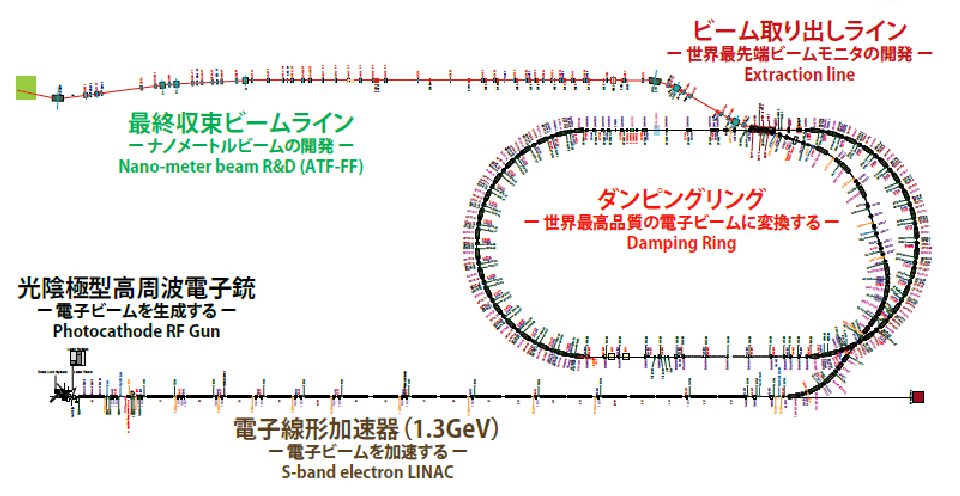
\includegraphics[angle=0,scale=0.50]{ATF_ATF2.png}\caption{Disposition of the Accelerator Test Facility (ATF), composed by a photocathode, a linac to 1.3GeV, a damping ring, an extraction line, the Final Focus (FF), and the beam dump.}\label{f:ATF_ATF2}
\end{subfigure}
\begin{subfigure}[b]{1.0\textwidth}
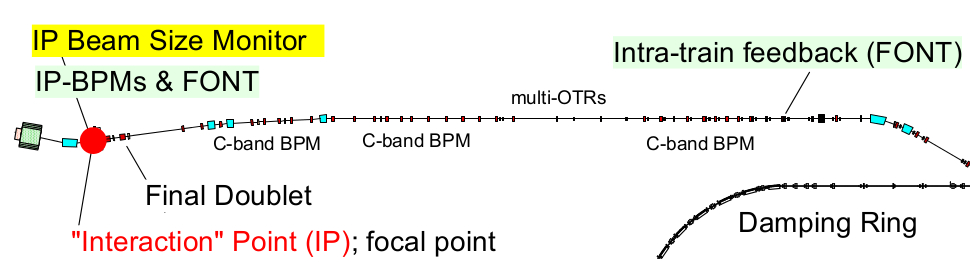
\includegraphics[angle=0,scale=0.65]{LigneATF2.jpg}\caption{Zoom over the extraction line, and Final Focus Section, highlighting the nominal Interaction Point location (IP). This region is known as ATF2.}\label{f:ATF2layout}
\end{subfigure}\caption{Diagrams containing the ATF composition and a zoom on the ATF2 section.}\label{f:ATF}
\end{figure}
The ATF2 lattice could be subdivided in two sections : the matching section and the Final Focus Section (FF). The first matches the beam extraction from the damping ring to the Final Focus in charge of beam size reduction.  In the FF, quadrupoles are located on individual movers to allow the beam steering and adjustment of relative alignment in X, Y and Roll angle. The top of Fig. \ref{f:FF_MADX} shows the lattice elements where the last point on the right corresponds to the nominal IP followed upstream by the QD0FF and QF1FF magnets, vertically and horizontally focusing each. These pair is called the Final Doublet (FD).\par
\begin{figure}[htb]
 \vspace*{-1.5cm}
 \begin{picture}(0,0)
 \put(386,-76){\tiny IP}
 \put(372,-44){\tiny QD0}
 \put(354,-44){\tiny QF1}
 \put(198,-44){\tiny QF7}
%  \put(195,-43){\tiny IM}
 \put(365,-76){\scriptsize FD}
 \put(70,-76){\scriptsize Matching Section}
 \put(220,-76){\scriptsize Final Focus Section (FF)}
 \put(138,-286){\tikz\draw[blue,dashed,thick] (0,0) -- (0,8.42);}
%  \put(220,-30){\tikz\draw[red,dashed,thick] (0,0) circle (0.4);}
%  \put(-90,20){\hbar}
\end{picture}
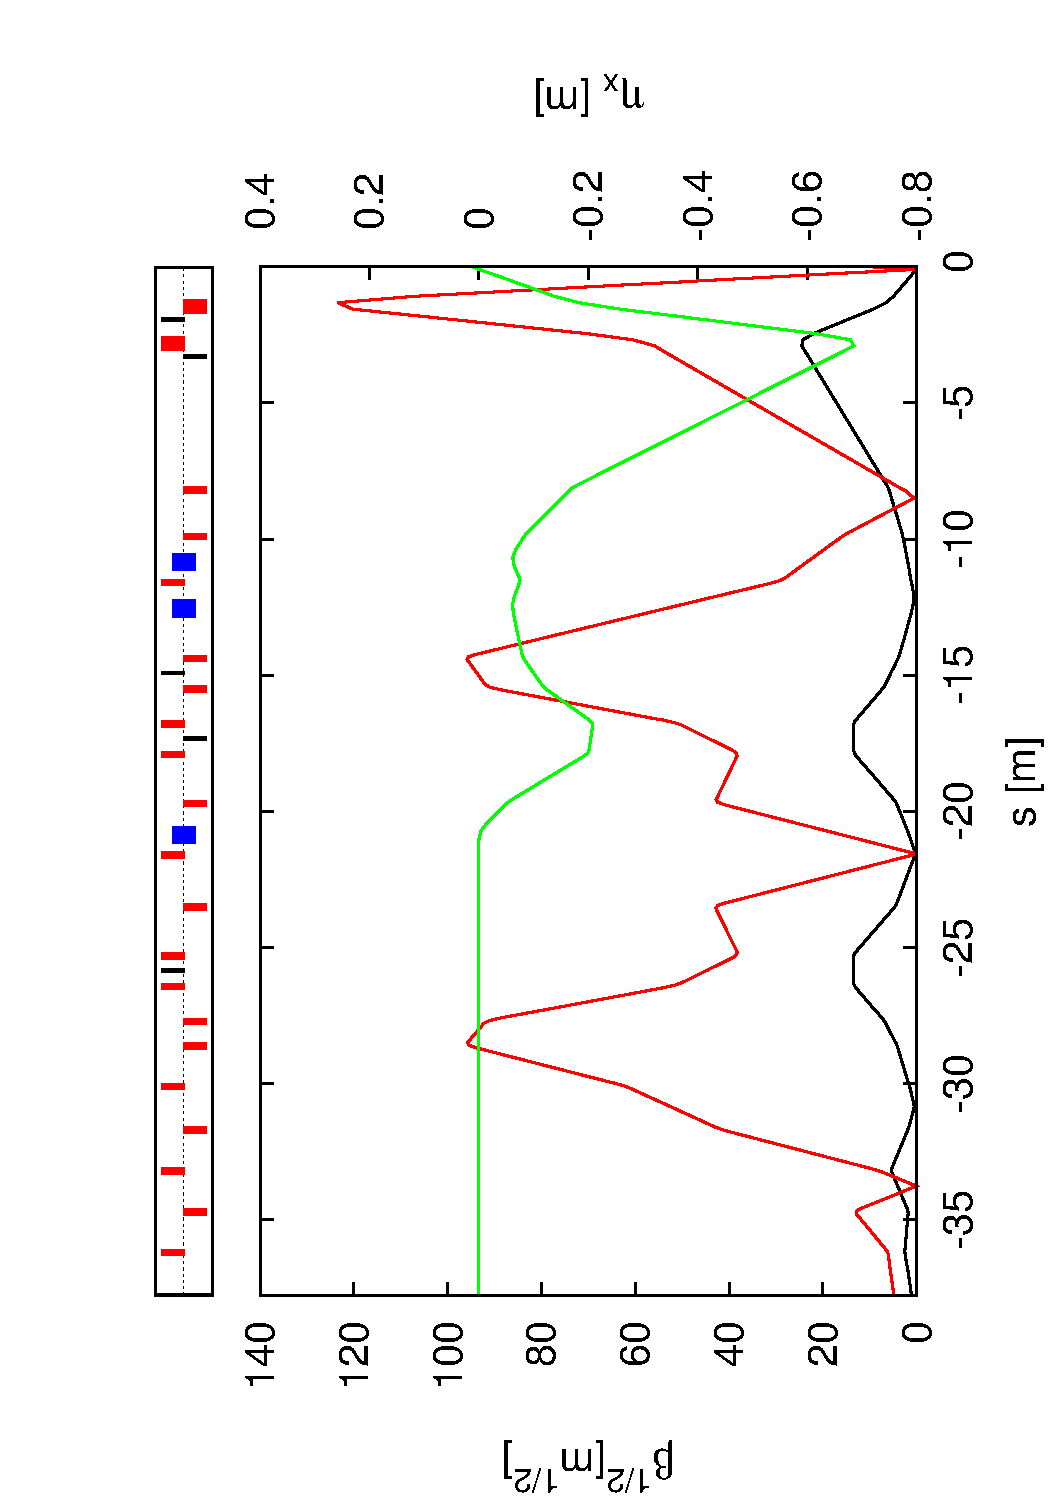
\includegraphics[angle=-90,scale=0.65]{lattice_ATF2_FF.pdf}\caption{Optical functions in the Final Focus Section at ATF2. On top is the ATF2 lattice : dipoles in blue, quadrupoles in red and sextupoles in black.}\label{f:FF_MADX}
\end{figure}
Below the lattice, Fig. \ref{f:FF_MADX} shows the vertical and horizontal $\beta$ functions reduction at QF7FF and the IP. This reduces the transfer matrix between these two points to the equivalent of a telescope with fixed magnification factor. The horizontal off-momentum function $\eta$ cancels at the IP, peaks in the FD region to correct chromaticity while it is reduced upstream in the sextupoles region. Additional chromaticity is created before QF7FF following the local-chromaticity correction method.

\section{Recent achievements and current work}
In 2014 vertical beam size about 55nm was observed at ATF2 \cite{Kubo50nm}, and since then smaller beam size can be achieved systematically down to 44nm \cite{KuboCLICws2015} demonstrating the local chromaticity correction method at charges below $0.1\times10^{10}$ particules per bunch.\par
The identified issue of intensity dependence is currently explored by the ATF2 collaboration. However, at low intensities the beam size remains above the designed 37nm. Possible contributions are: (1) the increase of the incoming beam emittance through out the ATF2 line, (2) systematic errors and resolution limitations on the beam size monitor, (3) beam drift beyond the tolerable margin and  (4) undetected optics mismatch.\par
Last two issues can be adressed by measuring the beam trajectory in the IP Region after the Final Doublet. In adittion, looking forward to \textbf{goal 2}, beam position measurement is a requirement for beam stabilization.\par
The work here described corresponds to the beam position monitors installed in 2013 by LAL in collaboration with Kyungpook National University (KNU), the Feedback in Nanosecond Timescale (FONT) group from Oxford, and the ATF2 staff.\par